\documentclass[20pt,landscape]{foils}
\usepackage{mbtslides}
\usepackage[english]{babel}
\usepackage{graphicx}
\usepackage{marvosym}
\usepackage{amssymb}  % provides \gtrsim
\usepackage{ellipse}
\usepackage{fancyvrb}
\usepackage{ulem}  % provides \sout
\usepackage[cm]{sfmath}

\newif\ifrubric
\rubricfalse

% This is supposed to make underscores cut'n'pastable
% Not sure what the lmodern package does or whether it's needed for this.
% But it's not working (though apparently it did in nam2023)
% \usepackage[T1]{fontenc}
% \usepackage{lmodern}
% \usepackage{textcomp}
% \DeclareTextSymbolDefault{\textunderscore}{T1}

\setlength{\unitlength}{1cm}


\newcommand{\bhref}[2]{\href{#1}{{\color{blue}#2}}}
\newcommand{\burl}[1]{{\color{blue}\url{#1}}}
\newcommand{\rfc}[1]{\bhref{https://www.rfc-editor.org/rfc/rfc#1}
                           {RFC\,#1}}

\newcommand{\buttimg}[1]
           {\mbox{\vtop{\vskip-2ex\hbox{\includegraphics[height=3ex]{#1}}}}}
\newcommand{\tcicon}[1]{
   \mbox{\vtop{\vskip-2.5ex\hbox{\includegraphics[height=3ex]{#1}}}}}
\newcommand{\buttitem}[1]{\item[{\makebox[0cm][r]{\tcicon{#1}}}]}
\definecolor{darkergreen}{rgb}{0,0.38,0}
\definecolor{purple}{rgb}{0.8,0,0.8}

% Fixes problem with includegraphics images screwing up colours on their
% page in the output PDF.  I have no idea *how* it fixes it mind.
\pdfpageattr {/Group << /S /Transparency /I true /CS /DeviceRGB>>}

% Oh no, this is required on my Ubuntu 22.04 (though not 20.04) installation
% to make the \ellipse commands work.
\makeatletter
\newdimen\@tempdimd
\makeatother

\begin{document}
\sf

\newcommand{\bigword}[1]{
  \vspace*{7cm}
  \begin{center}
    \color{darkblue}
    \scalebox{3}{
      \Huge\bf #1
    }
  \end{center}
  \addtocounter{page}{-1}
}

\ifrubric

\rightfooter{}
\MyLogo{}

\vspace*{3cm}
\hspace*{5cm}
\begin{minipage}{30cm}
\LARGE
\begin{enumerate}
  \item Wins
  \item Issues
  \item Matching with TOPCAT and STILTS
  \item AOB
\end{enumerate}
\end{minipage}

\newpage
\bigword{Wins?}
\newpage
\bigword{Issues?}
\newpage

\fi

\MyLogo{\color{grey}
        Mark Taylor, Crossmatching with TOPCAT and STILTS
        Bristol Astro Dev Group,
        17 January 2025}
\rightfooter{\quad{\color{grey}\thepage/\pageref*{lastPage}}}
\setcounter{page}{1}

\vspace*{1.0cm}
\begin{center}
{\color{darkblue}
\framebox{\Huge\bf
  \begin{minipage}{0cm}
  \begin{tabbing}
  Crossmatching with \\
  TOPCAT and STILTS
  \end{tabbing}
  \end{minipage}
}}
\\[2.0cm]
{\Large 
  Mark Taylor
}
\\[2.0cm]
{\large\color{grey}
  Bristol Astro Dev Group
  \\[2ex]
  17 January 2024
}
\end{center}

\vspace*{1.5cm}
\begin{center}
  \tiny
  \color{brown}
  \input gitid
\end{center}

\slide{Outline}

\begin{list1}
  \item What is crossmatching?
  \item Matching in TOPCAT
  \begin{list2big}
    \item Local matching function
    \item Using remote services
  \end{list2big}
  \item Using STILTS
  \item Demo
\end{list1}

\slide{Matching}

\begin{list0}
  \item What's crossmatching/why crossmatch?
  \begin{list2}
    \item Identify which rows in one table correspond to
                   which rows in another table
    \item ... typically in different observational regimes (e.g.\ wavelength)
    \item ... typically on basis of sky position (closest objects match)
    \item ... typically to combine observations,
              e.g.\ multi-wavelength photometry
  \end{list2}
  \item Typical science question:
  \begin{list2big}
    \item[] {\color{darkred}\sl
             Which sources from one observation correspond to
             which sources from another observation?}
  \end{list2big}
  \item Basic mathematical question:
  \begin{list2big}
    \item[] {\color{darkred}\sl
             Which positions in a list are close to
             which positions in another list?
             (for some definition of ``close to'')}
  \end{list2big}
  \item Conceptually straightforward ...
  \begin{list2big}
    \item for each position in one list, test each position in the other list
    \item write it yourself?
  \end{list2big}
  \item ... but there are complications
% \begin{list2big}
%   \item maybe use existing software
% \end{list2big}
\end{list0}

\newcommand{\matchfigSlide}[1]{
  \slide{Matching}
  \vspace*{0.5cm}
  \begin{center}
    \includegraphics[height=16cm]{#1}
  \end{center}
}
\matchfigSlide{match1.pdf}
\matchfigSlide{match2.pdf}
\addtocounter{page}{-1}
\matchfigSlide{match1.pdf}
\addtocounter{page}{-1}
\matchfigSlide{match3.pdf}
\addtocounter{page}{-1}
\matchfigSlide{match4.pdf}
\addtocounter{page}{-1}

\slide{Complications}

\begin{list1}
\vspace*{-0.2cm}
  \item Resource Usage
\vspace*{-0.2cm}
  \begin{list2}
    \item Algorithms that work nicely for 100 objects might be
          (much) too slow for 1,000,000 objects
\vspace*{-0.1cm}
    \item Memory usage can be an issue
  \end{list2}
\vspace*{-0.2cm}
  \item Spherical geometry
\vspace*{-0.2cm}
  \begin{list2}
    \item Careful when calculating distances for nearby objects (numerics)
\vspace*{-0.1cm}
    \item Careful near the antimeridian
\vspace*{-0.1cm}
    \item Careful near the poles
\vspace*{-0.1cm}
    \item How to chop the sky up into boxes?
  \end{list2}
\vspace*{-0.2cm}
  \item Other geometries
\vspace*{-0.2cm}
  \begin{list2}
    \item N-dimensional Cartesian spaces
\vspace*{-0.1cm}
    \item Sky + N-dimensional Cartesian spaces
  \end{list2}
\vspace*{-0.2cm}
  \item Different match criteria
\vspace*{-0.2cm}
  \begin{list2}
    \item Per-object error radius
\vspace*{-0.1cm}
    \item Elliptical/anisotropic match radius
  \end{list2}
\vspace*{-0.2cm}
  \item Related questions
\vspace*{-0.2cm}
  \begin{list2}
    \item Which objects {\sl don't\/} have any matches?
  \end{list2}
\vspace*{-0.2cm}
  \item Correctness
\vspace*{-0.2cm}
  \begin{list2}
    \item Are you sure you've got the right answer?
  \end{list2}
\end{list1}


\newcommand{\tcslide}[1]{
  \newpage
  \begin{picture}(32,0)
  \put(0,-19){
\includegraphics[height=19cm]{tclogo.pdf}}
  \put(21,-9){\begin{minipage}{16cm} #1 \end{minipage}}
  \end{picture}
}

\tcslide{}
\tcslide{
  \begin{list0}
    \item Get TOPCAT to do it for you!
    \begin{list2big}
      \item Local match functionality
      \item Talk to match-capable external services
    \end{list2big}
  \end{list0}
}
\addtocounter{page}{-1}

\slide{TOPCAT Local Matching Function}

\begin{picture}(30,0)
\put(23,-17){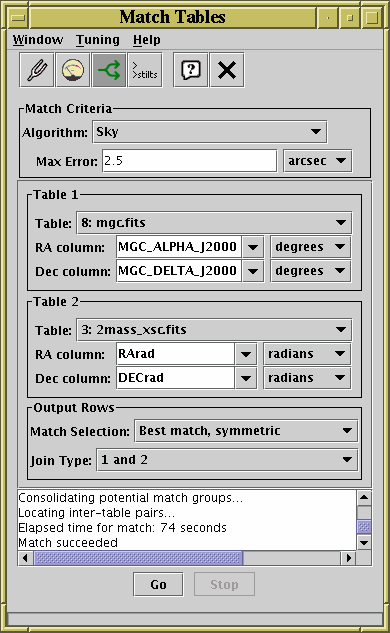
\includegraphics[height=17cm]{MatchWindow.png}}
\end{picture}
\vspace*{-1.5cm}

\begin{list0}
  \item TOPCAT can match tables you've loaded into it
  \begin{list2big}
    \item Use \buttimg{matchTwo2.png} {\bf Pair Match} window
    \begin{list3}
      \item (other windows in {\bf Joins} menu for
             matching 1 or 3, 4, 5, ... tables)
    \end{list3}
    \item Select match type, input tables etc and hit {\bf Go}
    \item Result is usually a new matched table
    \item Bonus: \buttimg{plotbutt1.png} button
  \end{list2big}
  \item Works well up to a few million rows
  \begin{list2big}
    \item though you can push it further with time and memory
  \end{list2big}
  \item Quite fast ($\lesssim$ couple of minutes)
  \item Quite flexible
  \begin{list2big}
    \item sky, Cartesian, exact, 3D, ellipses, errors, combinations, ...
  \end{list2big}
\end{list0}

\slide{TOPCAT for External Match Services}

\begin{picture}(30,0)
\put(24,-17){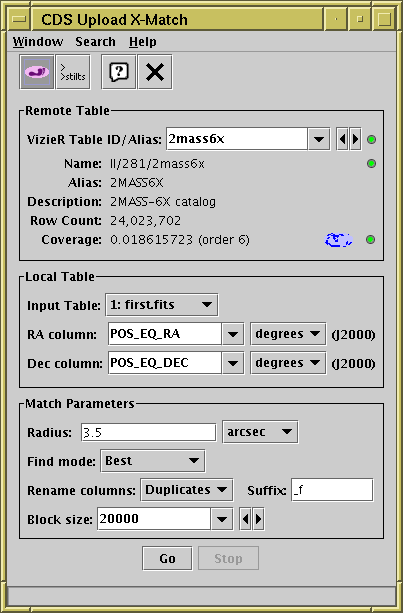
\includegraphics[height=17cm]{CdsUploadMatchWindow.png}}
\end{picture}
\vspace*{-1.5cm}

\begin{list0}
  \item TOPCAT can send a table you've loaded to a match service
  \item Works for external tables too large to load (e.g.\ large surveys)
  \item Usually best: {\bf CDS X-Match Service}
  \begin{list2big}
    \item Use \buttimg{xm3.png} {\bf CDS X-Match Upload} window
    \item Fill in remote (VizieR) table
    \begin{list3}
      \item Select from menu, or use
            \bhref{https://vizier.cds.unistra.fr/}{VizieR web page}
            to find ID
    \end{list3}
    \item Fill in local table, match criteria etc, hit {\bf Go}
    \item No size limit (TOPCAT chops up query into chunks for you)
    \item Usually pretty fast
    \begin{list2big}
      \item[] ... but sometimes slow or broken.
              Complain to \bhref{mailto:cds-question@unistra.fr}{CDS} or me.
    \end{list2big}
    \item May not have all the columns you want
  \end{list2big}
  \item Other options:
  \begin{list2big}
    \item TAP upload query (flexible, harder to use)
    \item Multi-cone search (slow, not generally recommended)
  \end{list2big}
  \item Result is a new matched table
\end{list0}

\slide{STILTS}

\vspace*{-0.2cm}
\begin{list0}
  \item STILTS is a set of command-line tools
  \begin{list2big}
    \item Does more or less all the same things as TOPCAT, but scriptably
\vspace*{-0.2cm}
    \item In some cases more scalable than TOPCAT
          (but generally not for matching commands)
\vspace*{-0.2cm}
    \item Can run it like:\\
          \hspace*{3em}
          {\color{brown}\verb|stilts <subcommand> arg=value arg=value ...|} \\
          or maybe: \\
          \hspace*{3em}
          {\color{brown}\verb|topcat -stilts <subcommand> arg=value arg=value ...|}
    \item Lots of documentation at
          \burl{http://www.starlink.ac.uk/stilts/sun256/}
  \end{list2big}
  \item STILTS matching commands:
  \begin{list2}
\vspace*{-0.2cm}
    \item[] \bhref{http://www.starlink.ac.uk/stilts/sun256/tskymatch2.html}
                  {\tt tskymatch2}: simple sky match 2 tables locally
\vspace*{-0.2cm}
    \item[] \bhref{http://www.starlink.ac.uk/stilts/sun256/tmatch2.html}
                  {\tt tmatch2}: flexible match 2 tables locally
\vspace*{-0.2cm}
    \item[] \bhref{http://www.starlink.ac.uk/stilts/sun256/tmatch1.html}
                  {\tt tmatch1}: match within a single table locally
\vspace*{-0.2cm}
    \item[] \bhref{http://www.starlink.ac.uk/stilts/sun256/tmatchn.html}
                  {\tt tmatchn}: match multiple tables locally
\vspace*{-0.2cm}
    \item[] \bhref{http://www.starlink.ac.uk/stilts/sun256/cdsskymatch.html}
                  {\tt cdsskymatch}: match local table with remote one
\vspace*{-0.2cm}
                                     using CDS X-Match service
    \item[] \bhref{http://www.starlink.ac.uk/stilts/sun256/tapskymatch.html}
                  {\tt tapskymatch}: match local table with remote one
                                     using TAP service
\vspace*{-0.2cm}
    \item[] \hspace*{2em} ... and a few others
  \end{list2}
\vspace*{-0.2cm}
  \item Example: \\
\vspace*{-0.2cm}
        {\color{brown}\small
        \begin{verbatim}
    stilts tmatch2 in1=obs_v.fits in2=obs_i.fits out=obs_iv.fits \
                   matcher=sky values1="ra dec" values2="ra dec" params=1.5
        \end{verbatim}}
\end{list0}

\newcommand{\ca}[1]{{\color{darkgreen}#1}}
\newcommand{\cb}[1]{{\color{teal}#1}}
\newcommand{\cc}[1]{{\color{hotpink}#1}}
\newcommand{\ccomm}[1]{{\color{black}#1}}
\begin{SaveVerbatim}[commandchars=\\\{\}]{filter-example}
stilts tmatch2 \ca{in1=obs_v.fits} \cb{in2=obs_i.fits} \cc{out=result.fits}
               matcher=sky values1='ra dec' values2='ra dec' params=1.5
               scorecol=DIST
               \ca{icmd1='select vmag<22'}                    \ccomm{# filter rows from input table 1}
               \cb{icmd2='addcol size hypot(ra_err,dec_err)'} \ccomm{# add a column to input table 2}
               \cc{ocmd='sort DIST' ocmd='head 100'}          \ccomm{# keep only 100 closest matches in output}
\end{SaveVerbatim}

\slide{STILTS Pipelines}

\begin{list0}
  \item You can do on-the-fly processing on (nearly) all STILTS input
        and output tables
  \begin{list2big}
    \item Use additional parameters like
          {\color{brown}\verb|cmd=<filter-command>|}
\vspace*{-0.2cm}
    \item Filters stack like a Unix pipeline
\vspace*{-0.2cm}
    \item Example:
    \begin{list3}
       \item[] {\color{grey} \UseVerbatim{filter-example}}
    \end{list3}
\vspace*{-0.5cm}
    \item There are lots of filters:
\vspace*{-0.2cm}
    \begin{list3}
      \item {\color{brown}\tt addcol},
            {\color{brown}\tt addskycoords},
            {\color{brown}\tt assert},
            {\color{brown}\tt badval},
            {\color{brown}\tt every},
            {\color{brown}\tt fixcolnames},
            {\color{brown}\tt keepcols},
            {\color{brown}\tt progress},
            {\color{brown}\tt repeat},
            {\color{brown}\tt rowrange},
          % {\color{brown}\tt sorthead},
            {\color{brown}\tt uniq},
            ...
      \item Or see the
            \bhref{http://www.starlink.ac.uk/stilts/sun256/filterSteps.html}
                  {full list}
    \end{list3}
  \end{list2big}
\vspace*{-0.2cm}
  \item There are options for what happens to output tables:
\vspace*{-0.2cm}
  \begin{list2big}
    \item Use {\color{brown}\verb|omode=<mode>|} parameter
\vspace*{-0.2cm}
    \begin{list3}
      \item {\color{brown}\tt omode=out} write table to file
            \ \ {\sl (default)}
      \item {\color{brown}\tt omode=topcat} load into running TOPCAT
      \item {\color{brown}\tt omode=count} count rows
      \item {\color{brown}\tt omode=stats} show statistics
      \item[] ... etc (see 
            \bhref{http://www.starlink.ac.uk/stilts/sun256/outModes.html}
                  {full list})
    \end{list3}
  \end{list2big}
\end{list0}

\newcommand{\interopSlide}[1]{
  \slide{TOPCAT/STILTS Interoperability}

  \begin{picture}(30,0)
    \linethickness{0.2cm}
    \put(18,-16){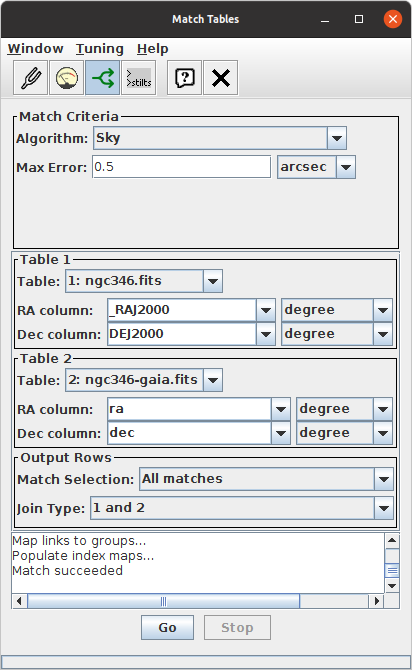
\includegraphics[scale=0.7]{PairMatchWindow.png}}
    #1
  \end{picture}
  \vspace*{-1.5cm}

  \begin{list0}
    \item Some TOPCAT windows can report \\
          equivalent STILTS command
    \begin{list2big}
      \item New since v4.10-2 (November 2024) \\
            --- you'll need a recent version
      \item Look for the \buttimg{stilts.png} {\bf STILTS} toolbar button
      \item Copy'n'paste text into shell
      \item ... sometimes needs a few adjustments
      \item Use \buttimg{stiltshelp.png} {\bf STILTS HELP} button \\
            for help on the command displayed
    \end{list2big}
  \end{list0}
}
\newcommand{\ifigStiltsbutt}{\put(21.4,-1.3){\color{red}\ellipse{1}{1}}}
\newcommand{\ifigStiltswin}{\put(26,-9){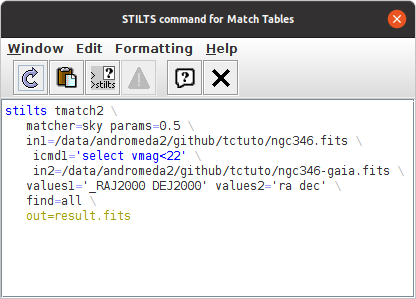
\includegraphics[scale=0.7]
                                         {PairMatch-stilts.png}}}
\newcommand{\ifigHelpbutt}{\put(28.6,-3.5){\color{red}\ellipse{1}{1}}}
\newcommand{\ifigHelpwin}{\put(17,-17){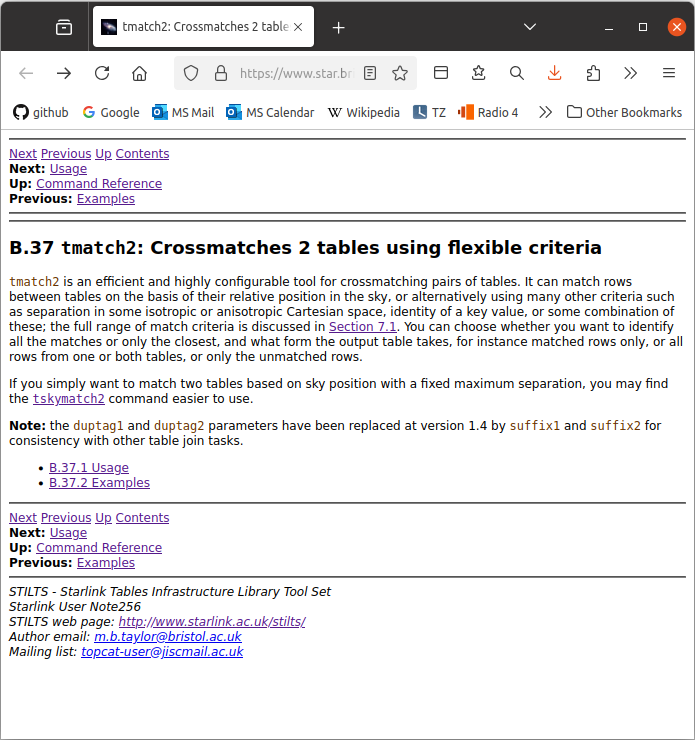
\includegraphics[height=14cm]
                                        {tmatch2-docs.png}}}
\interopSlide{}
\interopSlide{\ifigStiltsbutt}
\addtocounter{page}{-1}
\interopSlide{\ifigStiltsbutt \ifigStiltswin}
\addtocounter{page}{-1}
\interopSlide{\ifigStiltswin \ifigHelpbutt}
\addtocounter{page}{-1}
\interopSlide{\ifigStiltswin \ifigHelpwin}
\addtocounter{page}{-1}


\slide{TOPCAT/STILTS Matching Limitations}

\begin{list0}
  \item Scalability
  \begin{list2}
    \item TOPCAT local matching doesn't work so well for large catalogues
    \begin{list3}
      \item $N \lesssim 10^{7}$ usually OK, more than that may need more memory
    \end{list3}
    \item Can get into trouble with lots of positions close together
    \item Symptoms of failure: match runs very slowly/grinds to a halt
  \end{list2}
  \item Functionality
  \begin{list2}
    \item None of these techniques do anything very clever:
          just find pairs satisfying match criteria
    \item You might want other answers
    \begin{list3}
      \item Probability of a real association
      \item ... given additional constraints like colour/magnitude/spectrum
      \item ... given local environment (e.g.\ source density)
      \item Matching observations with widely different resolutions
      \item Matching points to extended sources
      \item 1:N matches
      \item True associations between $N>2$ tables
    \end{list3}
  \end{list2}
\end{list0}

\slide{Summary/Tips}

\begin{list0}
  \item Smallish tables:
  \begin{list2big}
    \item Use TOPCAT match window,
          or STILTS {\color{brown}\tt tmatch*} commands
  \end{list2big}
  \item Smallish table {\sl vs.\/} large survey
  \begin{list2big}
    \item Use TOPCAT CDS Upload X-Match window,
          or STILTS {\color{brown}\tt cdsskymatch} command
    \item Or maybe a TAP upload query or multi-cone if that's no good
  \end{list2big}
  \item Examine match results --- they may not mean what you think
  \begin{list2big}
    \item Plot associations on the sky (or relevant space)
    \item Look at separation statistics, e.g.\ plot histograms
    \item Careful of crowded fields, best-only results
  \end{list2big}
  \item TOPCAT can tell you what STILTS command to use
  \item Extended TOPCAT crossmatching talk from 2021 is available:
        \bhref{https://youtu.be/mdMtmy3Zq-Q&t=3582s}{video} and
        \bhref{https://www.star.bristol.ac.uk/mbt/talks/shristi2021/}{materials}
\end{list0}

\vspace{0.2cm}
\begin{center}
  {\color{darkred}\Huge\bf\sl Thanks!}
\end{center}

\label{lastPage}

\ifrubric

\newcommand{\aobSlide}[1]{
\newpage
\rightfooter{}
\MyLogo{}
\begin{picture}(30,0)
  #1
\end{picture}
\bigword{AOB?}
}
\aobSlide{}
\aobSlide{
  \put(25.6,-19.2){
\includegraphics[height=3.5cm]{spam.jpg}}
  \put(31,-19){
\includegraphics[height=5cm]{beans.jpg}}
  \put(24.7,-18.8){
\includegraphics[height=6cm,angle=-15]{wkd.png}}
}
\aobSlide{}

\fi

\end{document}

% $Id: sql.tex,v 1.17 2024/05/03 11:56:03 mbt Exp $
